\section{Description}

This is a lab report of the second given mandatory assignment in the course control systems engineering 2022. The assignment is answered by students at NTNU Ålesund, November 2022.

A servo motor is connected to a balance beam via a lever-arm. Adjusting the servo position will adjust the angle, $\alpha$, between the horizontal plane and the balance beam. An infrared sensor, hereby referred to as IR-sensor, is mounted to one end of the beam. The sensor is connected to an Arduino micro controller to measure the distance to a rolling ball on the balance-beam. The goal is to make the ball stay at a predetermined position on the balance beam by regulating the servo-position and thereby the angle of the balance-beam. A complete list of components, variables and model is given below.

All given values and variables of the system:


\begin{tabular}{ll}
Beam length:                           & L = 0.4m\\
Motor-center to lever-arm:             & d = 0.06m\\
Angel between lever arm and disc:      & $\theta$\\
Distance between ball and sensor:      & 0.1m $\leq$ r $\leq$ 0.3m\\
Diameter of ball:                      & R = 0.04m\\
Angel between lever and beam:          & $\beta$\\
Height of lever arm:                   & h = 0.09m\\
Angel between beam and bottom plate:   & $\alpha$\\
\end{tabular}                             

List of components:

\begin{tabular}{ll}
    Sensor: SHARP 2Y0A21 with RS code: 666-6564\\
    Servo motor: Parallax S148 Standard Servo with RS code: 781-3058\\
    Controller: Arduino Uno Rev3\\
    Capacitors: 22$\mu$F, 330nF, 100nF\\
    Voltage regulator: L7805CV with RS code: 918-1971
\\
    
    
    

\end{tabular}
    
\begin{figure}[h]
    \centering
    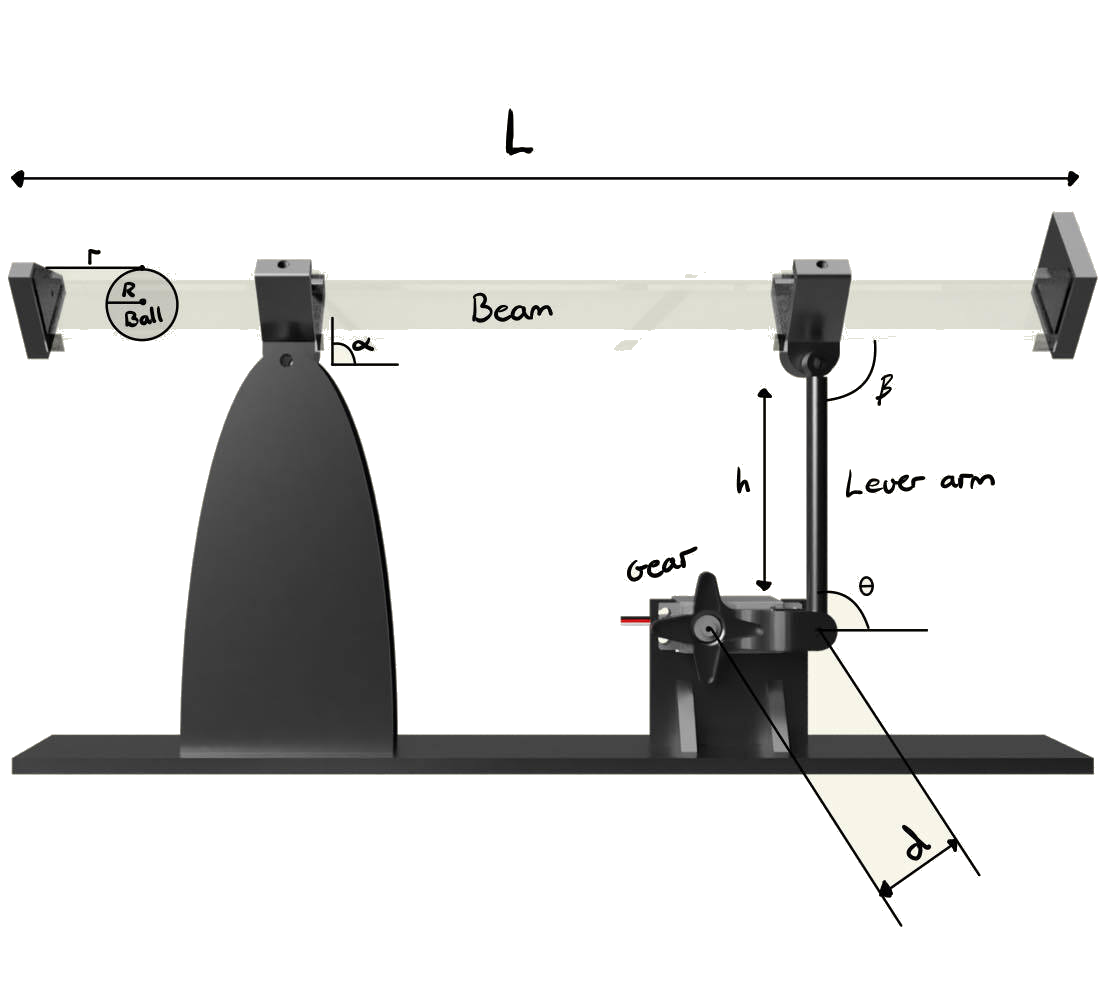
\includegraphics[width = 0.8\textwidth]{Images/3D-MAIN.png}
    \caption{3D rendered model of the physical system with given variables}
    \label{fig:3d-model}
\end{figure}

